\documentclass[12pt]{article}%

\usepackage{fancyhdr}
\pagestyle{fancy}
\fancyhf{}
\fancyhead[R]{\thepage}

\usepackage{cmap}				
\usepackage{mathtext} 
\usepackage{listings}

\usepackage{biblatex}
\addbibresource{lib.bib}

\usepackage{euscript}
\usepackage{mathrsfs}

\usepackage[T2A]{fontenc}
\usepackage[utf8]{inputenc}
\usepackage[english,russian]{babel}
\usepackage{amsmath,amsfonts,amssymb,amsthm,mathtools}

\setlength\fboxsep{3pt}
\setlength\fboxrule{1pt}

\usepackage{graphicx}
\usepackage{hyperref}
\usepackage[usenames,dvipsnames,svgnames,table,rgb]{xcolor}
\usepackage{wrapfig}
\hypersetup{				
    unicode=true,           
    pdftitle={Заголовок},   
    pdfsubject={Тема},      
    pdfkeywords={keyword1} {key2} {key3},
    colorlinks=true,
    linkcolor=black,
    citecolor=black,
    filecolor=magenta,
    urlcolor=cyan
}

% Работа с Python
\usepackage{minted}
\definecolor{LightGray}{gray}{0.98}

% Работа с enumerate
\usepackage{enumitem}

% Для удобной работы с плавающими объектами
\usepackage{placeins}

\newcommand*{\Title}{\begingroup
\centering 

\large {Федеральное автономное образовательное учреждение высшего образования}
\vspace*{\baselineskip}

\large {«Национальный исследовательский университет «Высшая школа экономики»»}
\vspace*{\baselineskip}

\vspace*{\baselineskip}
\large{\textbf{Отчет по лабораторной работе 2}}

\vspace{0.1cm}
\large{Решение систем линейных алгебраических уравнений прямыми методами, теория возмущений.}

\vspace{0.2cm}
\large{Вариант 10: задачи 3.1.10, 3.4, 3.6.2}

\vspace{1.5cm} 

\begin{flushright}
  \textbf{\normalsize Выполнил:}
  
  \vspace{0.3cm} 
  {\normalsize Студент группы БПМ-211}
  
  {\normalsize Ляхов Артём Андреевич}

\end{flushright}


\vspace{0.2cm}  
\begin{flushright}
  \textbf{\normalsize Преподаватель:} 

  \vspace{0.2cm}

 {\normalsize Брандышев Петр Евгеньевич}
 
\end{flushright}

\vfill
\date{}{Февраль 2024 г.}



\endgroup\clearpage}

\begin{document}
\Title
\tableofcontents
\newpage

\section{Задача 3.1.10. Оценка погрешности решения СЛАУ в зависимости от погрешности правой части}

\subsection{Формулировка задачи}
Дана система линейных алгебраических уравнений $Ax = b$ порядка $n$. Необходимо исследовать зависимость погрешности решения $x$ от погрешностей правой части системы $b$.

Значения $a_{ij}$ матрицы $A$ и $b_i$ вектора $b$ задаются следующими соотношениями:
\begin{equation*}
    a_{ij} = \sin\left(\frac{c_{ij}}{8}\right),\ \ \ 
    c_{ij} = 0.1\cdot N \cdot i \cdot j,\ \ \ 
    b_i = N
\end{equation*}
где $N = 10$ - номер варианта, $n=5$ - порядок системы.

\subsection{Теоретический материал}
Пусть $A$ - квадратная матрица порядка $n$, тогда будем называть \textit{числом обусловленности} матрицы $A$ величину:
\begin{equation*}
    cond(A) = ||A^{-1}||\cdot ||A||
\end{equation*}

В общем случае в качестве нормы $||\cdot||$ может выступать любая матричная норма. В рамках нашей задачи мы будем использовать $\infty$-норму:
\begin{equation}
    ||A||_{\infty} = 
    \max\limits_{1 \leqslant i \leqslant n}\sum\limits_{j=1}^{n}|A_{ij}|
\end{equation}

Таким образом, в рамках нашей задачи:
\begin{equation}
    cond(A) = ||A^{-1}||_{\infty} \cdot ||A||_{\infty} 
\end{equation}

Пусть $x$ - точное решение системы линейных алгебраических уравнений $n$-го порядка, $x^{*}$ - приближённое решение, тогда относительная погрешность $x^{*}$ может быть найдена с использование векторной нормы $||\cdot||_{\infty} = \max\limits_{1 \leqslant i \leqslant n}|x_i|$ 
через соотношение:
\begin{equation}
    \delta(x^{*}) = \frac{||x - x^{*}||_{\infty}}{||x||_{\infty}}
\end{equation}

Предположим, что правая часть СЛАУ задана приближённо и мы нашли решение $x^{*}$ для приближённой правой части $b^{*}$. В этом случае для $x^{*}$ верно следующее неравенство:
\begin{equation}
    \delta(x^{*}) \leqslant cond(A) \cdot \delta(b^{*})
\end{equation}

\subsection{Порядок решения задачи}
1)Задать матрицу системы $A$ и вектор правой части $b$. Используя встроенную функцию, найти решение системы $x$ системы $Ax=b$ с помощью метода Гаусса.
\newline
2)С помощью встроенной функции вычислить число обусловленности матрицы $A$.
\newline
3)Принимая решение $x$, полученное в п.1, за точное, вычислить вектор $d = (d_1, \dots d_n)^{T}$, где 
\[
d_i = \frac{||x - x^{i}||_{\infty}}{||x||_{\infty}} 
\]
$i = 1,\dots, n$, относительных погрешностей решений $x^{i}$ систем $Ax^{i} = b^{i}$, и где компоненты вектора $b^{i}$ вычисляются по формулам:
\[
b^{i} = \begin{cases}
            b_k + \Delta,\ \ k=i, \\
            b_k, \ \ k \ne i
        \end{cases}
\]
\newline
($\Delta$ - произвольная величина погрешности). 
\newline
4)На основе вычисленного вектора $d$ построить гистрограмму. По гистрограмме определить компоненту $b_m$, которая оказывает наибольшее влияние на погрешность решения. 
\newline
5)Оценить теоретически погрешность решения $x^m$ с помощью следующего соотношения:
$\delta(x^m) \leqslant cond(A) \cdot \delta(b^m)$. Сравнить значение $\delta(x^m)$ со значением практической погрешности $d_m$. 


\subsection{Код программы}
Код программы для численного эксперимента можно найти в jupyter-ноутбуке, прикреплённом вместе с этим отчётом.

\subsection{Результаты вычислительного эксперимента}
\begin{table}[h]
    \centering
    \begin{tabular}{|c|c|c|c|c|}
    
    \hline $d_1 $  &  $d_2$  &  $d_3$  &  $d_4$  &  $d_5$  \\
    \hline 0.1529  & 0.1807  & 0.1075  & 0.0345  & 0.0048  \\
    \hline
    \end{tabular}
    \caption{Получившийся вектор $d$. Все значения было округлены до 4 знаков после запятой. Вычисления проводились для $\Delta=0.5$.}
    \label{tab:d_vec}
\end{table}
\FloatBarrier

\begin{figure}[h]
    \centering
    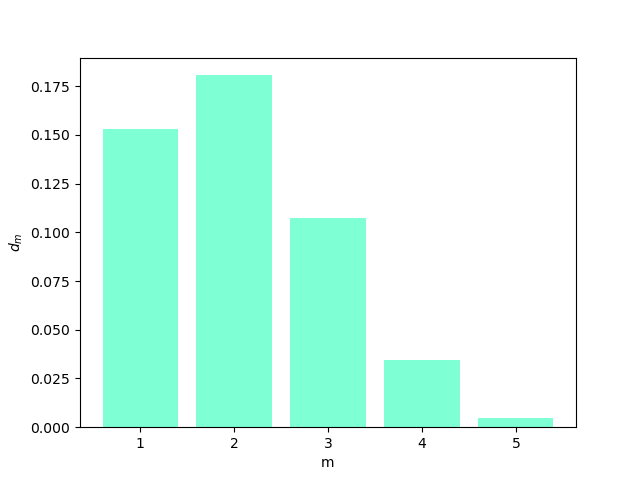
\includegraphics[width=\linewidth]{problem1_precision.png}
    \caption{Гистограмма относительной погрешности решения в зависимости от номера компоненты $m$.}
    \label{fig:d_vec}
\end{figure}
\FloatBarrier

\textbf{Вывод:} из таблицы \ref{tab:d_vec} и гистрограммы \ref{fig:d_vec} мы наблюдаем, что наибольшее влияние на погрешность решения системы уравнений оказывает компонента $b_2$.

\begin{table}[h]
    \centering
    \begin{tabular}{|c|c|}
        \hline $m$                                      & 2             \\
        \hline $cond(A)$                                & 7690516.4277  \\
        \hline $\delta(b^m)$                            & 0.05          \\
        \hline $d(x^m)$                                 & 0.1807        \\
        \hline $\delta(x^m) = cond(A) \cdot \delta(b^m)$ & 384525.8214  \\
        \hline
    \end{tabular}
    \caption{Результаты вычислений погрешностей для компоненты $b_2$. Все значения были округлены до 4 знаков после запятой. Неравенство $d(x^m) \leqslant \delta(x^m)$ принимает вид: $0.1807 \leqslant 384525.8214$.}
    \label{tab:my_label}
\end{table}
\FloatBarrier
\textbf{Вывод:} теоретическая оценка погрешности сверху (обозначенная за $\delta(x^m)$) на несколько порядков больше, чем практическая. Это объясняется тем, что современные численные методы нахождения решений системы уравнений очень точны.


\newpage
\section{Задача 3.4. Решение СЛАУ с использованием $LU$-разложения матрицы}
\subsection{Формулировка задачи}
Требуется решить систему уравнений $Ax=b$ из \textit{задачи 3.1}, используя $LU$-разложение матрицы $A$.
\subsection{Теоретический материал}
Пусть $A$ -  невырожденная матрица порядка $n$, сформулируем теорему:
\newline
\textbf{Теорема.} Если все главные миноры $A$ отличны от нуля, то существуют такие нижнетреугольная $L$ с единицами на главной диагонали и верхнетреугольная $U$ квадратные матрицы, что $A = LU$.

Рассмотрим систему уравнений $Ax=b$. Предположим, что нам известно $LU$-разложение матрицы, то есть исходную систему можно переписать в виде:
\begin{equation*}
    LUx = b
\end{equation*}
Решение задачи в таком виде сводится к двум шагам.

Первый шаг, называемый \textit{прямой заменой}, состоит в том, чтобы решить вспомогательную систему
\begin{equation}\label{eq:LU_sys1}
    Ly = b
\end{equation}
относительно вектора $y$. 

Поскольку $L$ - нижнетреугольная матрица с единицами на главной диагонали, то решение системы \ref{eq:LU_sys1} может быть выражено в явном виде:
\begin{equation}\label{eq:LU_sol1}
    y_{i} = b_{i} - \sum\limits_{k=1}^{i-1}l_{ik} \cdot y_{k}
\end{equation}

Второй шаг, называемый \textit{обратной заменой}, заключается в нахождении искомого вектора $x$ из системы:
\begin{equation}
    Ux = y
\end{equation}
Так как $U$ - верхнетреугольная матрица, то компоненты вектора $x$ могут быть выражены явно через соотношения:
\begin{equation}\label{eq:LU_sol2}
    x_{i} = \frac{1}{u_{ii}}\left(
    y_{i} - \sum\limits_{k=i+1}^{n} u_{ik} \cdot  x_{k}
    \right)
\end{equation}

В случае если хотя бы один из главных миноров $A$ равен нулю, мы можем воспользоваться утверждением:
\newline
\textbf{Утверждение.} Если $A$ - невырожденная матрица, то существует перестановочная матрица $P$ такая, что все главные миноры матрицы $PA$ отличны от нуля.

Таким образом, мы можем домножить обе части системы $Ax=b$ на матрицу $P$ и к получившейся системе применить все рассуждения выше.



\subsection{Порядок решения задачи}
1. Реализуем функцию \textbf{lu}(A), которая принимает на вход матрицу $A$ и возвращает матрицы $P$, $L$, $U$.
\newline
2. С помощью формул \ref{eq:LU_sol1} и \ref{eq:LU_sol2} для правой части $P \times b$ находим решение системы $x$.



\subsection{Код программы}
\begin{minted}[
frame=single,
framesep=10pt,
framerule=0.1pt,
bgcolor=LightGray
]{python}
def lu(A: np.ndarray):
    """
    Computes LU decomposition of matrix with partitial 
    pivoting

    :param np.ndarray A: array to decompose. Must be 
    2-dimensional and be square matrix.
    :return: P, L, U matrices: P - permutation matrix, 
                               L - lower triangular matrix, 
                               U - upper triangular matrix.
    """
    n = A.shape[0]

    U = A.copy()
    L, P = np.eye(n, dtype=float), np.eye(n, dtype=float)

    for i in range(n):
        # Partitial pivoting
        for k in range(i, n):
            if ~np.isclose(U[i, i], 0.0):
                break
            U[[i, k]] = U[[k, i]]
            P[[i, k]] = U[[k, i]]
        
        factor = U[i+1:, i] / U[i, i]
        L[i+1:, i] = factor
        U[i+1:] -= factor[:, None] * U[i]
    
    return P, L, U
\end{minted}


\begin{minted}[
frame=single,
framesep=10pt,
framerule=0.1pt,
bgcolor=LightGray
]{python}
def forward_substitution(L, b):
    """
    Returns a solution y of linear system Ly = b, aka
    performs forward substitution in solution 
    of system LUx=b.

    :param np.ndarray L: lower-triangular matrix L 
    from LU-decomposition.
    :param np.ndarray b: vector - right part of system Ax=b 
    or LUx=b.
    :return np.ndarray: solution of the system Ly=b. 
    """
    n = L.shape[0]
    y = np.zeros(n, dtype=float)
    for i in range(n):
        y[i] = (b[i] - L[i, :i] @ y[:i]) / L[i, i]
    return y
\end{minted}


\begin{minted}[
frame=single,
framesep=10pt,
framerule=0.1pt,
bgcolor=LightGray
]{python}
def back_substitution(U, y):
    """
    Returns a solution of linear system Ux = y, aka 
    performs back substitution in solution of linear system 
    LUx = b.

    :param np.ndarray U: upper-triangular matrix U 
    from LU-decomposition.
    :param np.ndarray y: solution of system 
    Ly=b (see forward_substitution).
    :return np.ndarray: solution of the system Ux=y, aka 
    solution of system LUx=b.
    """
    
    n = U.shape[0]
    x = np.zeros(n, dtype=float)
    for i in reversed(range(n)):
        x[i] = (y[i] - U[i, i+1:] @ x[i+1:]) / U[i, i]
    return x
\end{minted}


\begin{minted}[
frame=single,
framesep=10pt,
framerule=0.1pt,
bgcolor=LightGray
]{python}
def solve_lu(A, b):
    """
    Solves a system of linear equations using 
    LU-decomposition.

    :param np.ndarray A: coefficient matrix.
    :param np.ndarray b: ordinate or 
    “dependent variable” values.
    :return np.ndarray: solution to the system Ax=b. 
    """
    n = A.shape[0]
    P, L, U = lu(A)

    b = P @ b
    y = forward_substitution(L, b)
    return back_substitution(U, y)
\end{minted}


\subsection{Результаты вычислений}
\begin{table}[h]
    \centering
    \begin{tabular}{|c|c|}
        \hline  Переменная & Значение \\
        \hline  $x_1$      & 1732046.00043  \\
        \hline  $x_2$      & -2052111.2245  \\
        \hline  $x_3$      & 1226346.7732   \\
        \hline  $x_4$      & -395911.89193  \\
        \hline  $x_5$      & 55377.4694     \\
        \hline
    \end{tabular}
    \caption{Решение системы из задачи 3.1.10, найденное с использованием $LU$-разложения матрицы $A$. Относительная погрешность найденного решения $\delta \approx 7 \cdot 10^{-11} $.}
\end{table}

\textbf{Вывод:} Как мы видим, решения найденные в рамках задачи 3.1.10 и с помощью $LU$-разложения матрицы $A$ практически совпали.
\newpage





\newpage
\section{Задача 3.6.2. Исследование зависимости решения системы линейных уравнений от вычислительной погрешности}
\subsection{Формулировка задачи}
Дана система уравнений $Ax=b$ порядка $n$, где $A = A(t)$, $t$-параметр. Необходимо исследовать зависимость решения системы $Ax=b$ от вычислительной погрешности при заданных значениях параметра $t$.

Значения $A_{ij}$ матрицы $A$ задаются соотношением:
\[
A_{ij} = \begin{cases}
            q_{M}^{j},\ \ i \ne j \\
            q_{M}^{j} + t,\ \ i = j
        \end{cases}
\]
где $q_{M} = 0.993 + (-1)^M \cdot M \cdot 10^{-4}$, параметр $t$ принимает значения $\{0.0001,\ 1,\ 10000\}$. 

Элементы вектора $b$ вычисляются по формуле $b_{j} = q_{M}^{n+1-j}$. Согласно условию варианта $M=2$, $n=100$, $m=5$.


\subsection{Порядок решения задачи}
1)Составить программу, реализующую метод Гаусса (схема частичного выбора) для произвольной системы $Ax=b$. Используя составленную программу, найти решение заданной системы $Ax=b$.
\newline
2)Составить программу округления числа до $m$ знаков после запятой. Вычислить элементы матрицы $A$ и вектора $b$ по формулам, представленным в формулировке задачи, производя при этом округление до $m$ знаков после запятой. Подобным образом будут получены матрица $A_{1}$ и вектор $b_{1}$.
\newline
3)Решить систему уравнений $A_{1}x=b_{1}$ методом, указанным в п.1, обращаясь каждый раз к программе округления. Оценить практически погрешность полученного решения.
\newline
4)Сравнить результаты, полученные при различных параметра $t$.

При этом в качестве абсолютной погрешности будем использовать 1-норму разности:
\[
\Delta(x^1) = ||x - x^1 ||_1 = 
\sum\limits_{i=1}^{n}|x_{i} -  x_{i}^1|,
\]
а в качестве относительной погрешности:
\[
\varepsilon(x^1) = \frac{\Delta(x^1)}{||x||_1} = 
\frac{
\sum\limits_{i=1}^{n}|x_i - x_i^1|
}{
\sum\limits_{i=1}^{n}|x_i|
}
\]


\subsection{Код программы}
Ниже представлена программная реализация метода Гаусса для решения системы уравнений на языке программирования Python:
\begin{minted}[
frame=single,
framesep=10pt,
framerule=0.1pt,
bgcolor=LightGray
]{python}
def solve_gauss(A, b, m = None):
    """
    Solves a system of equations by the Gauss method.

    :param np.ndarray A: coefficient matrix.
    :param np.ndarray b: ordinate 
    or "dependent variable" values.
    :return np.ndarray x: solution to the system Ax=b.
    """
    n = A.shape[0]
    a = np.concatenate((A, b.reshape(-1, 1)), axis=1)

    for i in range(n):
        j = np.argmax(np.abs(a[i, i:-1])) + i
        a[[i, j]] = a[[j, i]]

        if np.isclose(a[i, i], 0):
            continue

        for k in range(i+1, n):
            ratio = a[k, i]/a[i, i]
            a[k] = a[k] - ratio * a[i]

        if m is not None:
            a = np.round(a, m)
    
    x = np.zeros(n, dtype=float)
    for i in reversed(range(n)):
        value = (a[i, -1] - x[i+1:] @ a[i, i+1:-1])/a[i, i]
        x[i] = value if m is None else np.round(value, m)

    return x
\end{minted}
\FloatBarrier

Код для проведения вычислительного эксперимента можно найти в jupyter-ноутбуке, прикреплённом вместе с этим отчётом.


\subsection{Результаты вычислительного эксперимента}
\begin{table}[h]
    \centering
    \begin{tabular}{|c|c|c|c|}
    \hline             & t=0.0001 & t=1 & t=10000  \\
    \hline $\Delta(x^1)$       & $7.47 \cdot 10^{-4}$ 
                               & $7.28 \cdot 10^{-4}$ 
                               & $7.28 \cdot 10^{-4}$ \\
    \hline $\varepsilon(x^1)$  & $5.3 \cdot 10^{-6}$  
                               & $5.21 \cdot 10^{-6}$
                               & $5.24 \cdot 10^{-6}$ \\
    \hline
    \end{tabular}
    \caption{Абсолютная и относительная погрешности решения, полученного с использованием округления до $m=5$ знаков после запятой, при различных значениях параметра $t$.}
    \label{tab:my_label}
\end{table}

\textbf{Вывод:} как мы видим, практическая погрешность решения системы $Ax=b$ зависит только от вычислительной погрешности и не зависит от параметра $t$.


\end{document}